\section{Methodology}
To date (Jan 1st 2021), authors did not release their code. Therefore, we fully re-implement the Hamiltonian architecture, the integrators, and the simulated environments. To further evaluate the system, we implement two additional environments and one additional integrator. We developed our implementation in Python3 using PyTorch \cite{pytorch} machine learning library for the Hamiltonian architecture and the Scipy \cite{scipy} ODE solver for the simulated environments, as well as OpenCV \cite{opencv_library} for image manipulation.
Our code can be found in this \href{https://github.com/CampusAI/Hamiltonian-Generative-Networks}{repository}\footnote{https://github.com/CampusAI/Hamiltonian-Generative-Networks}. We run most of the experiments using an NVIDIA GeForce RTX 2080Ti and some on an NVIDIA GTX 970.  


\subsection{Hamiltonian Generative Network (HGN)}
% \todo{Make sure all important information is stated here (e.g. no relu in hnn, shapes(?))}

The HGN \cite{hgn} architecture can be split into two high-level components. The first (Figure \ref{fig:initial_cond}) reads the initial $k+1$ frames of an environment rollout and extracts the abstract positions and momenta $(\bm{q}_k, \bm{p}_k)$ correspondent to the $k$-th step. Second, a recurrent model takes $(\bm{q}_k, \bm{p}_k)$ as first input and performs integration steps of a fixed $\Delta t$, predicting the evolution of the system in terms of abstract positions and momenta \footnote{In addition, we test how the network performs when trained as an autoencoder, ie: fit the complete sequence and reconstruct it. (Section \ref{sec:reproduction}) }. For each step, the abstract position is decoded into an RGB image. As figures \ref{fig:initial_cond}, \ref{fig:unroll} depict, this model is composed by four main networks:

\begin{itemize}
    \item \textbf{Encoder}: Parametrized by: $\phi$. 8-layer 64-filter Conv2D network with ReLU activations that takes a sampled video rollout from the environment and outputs the mean and variance of the encoder distribution $q_\phi (\bm{z})$ parametrized as a diagonal Gaussian with prior $p(\bm{z}) = \mathcal{N}(\bm{0}, \mathbb{I})$. The latent variable $\bm{z}$ is sampled from $q_{\phi}$ with the reparametrization trick \cite{vae}. The input of this layer is constructed by concatenating all the rollout frames in the channel axis. Therefore, if working with RGB images, the input has shape: $H \times W \times 3 \cdot N$. Where $H, W, N$ are Height, Width, and Number of frames, respectively. 
    % \todo{Shape?}
    \item \textbf{Transformer}: Parametrized by: $\psi$. Takes in the sampled latent variable $\bm{z}$ and transforms it into a lower-dimensional initial state $\bm{s}_k = (\bm{q}_k, \bm{p}_k)$, by applying 3 Conv2D layers with ReLU activations, stride 2, and 64 filters.
    % \todo{Shape?}
    \item \textbf{Hamiltonian}: Parametrized by: $\gamma$. It is a 6-layer 64-filter Conv2D network with SoftPlus activations which takes in the abstract positions and momenta $(\bm{q}_t, \bm{p}_t)$ and outputs the energy of the system $e_t \in \mathbb{R}$. This network is used by the integrator (Section \ref{sec:integrators}) to compute the system state at the next time-step $(\bm{q}_{t+1}, \bm{p}_{t+1})$ exploiting Eq. \ref{eq:hamilton}. Since Eq. \ref{eq:hamilton} involves partial derivatives of $\mathcal{H}$ w.r.t. $\bm{q}$ and $\bm{p}$, the training process involves second-order derivatives of the Hamiltonian network weights. For this reason, SoftPlus activations are used instead of ReLU. 
    \item \textbf{Decoder}: Parametrized by: $\theta$. 3-residual block upsampling Conv2D network (as in \cite{karras2018progressive}) which converts the abstract position $\bm{q}_t$ into an image close to the source domain.
\end{itemize}

Given an input sequence: $(\bm{x}_0, ..., \bm{x}_T)$ and a value $k + 1$ of input-length, the loss function
\footnote{The formulation of the loss in Eq. \ref{eq:loss} particularly w.r.t. the distribution $q_{\phi}$ is different from that of the paper\cite{hgn} where it was written as $q_{\phi}(\bm{z} \vert \bm{x}_0, ..., \bm{x}_T)$, which initially led us to think that the encoder had access to the whole rollout. Discussion with the authors clarified that the encoder reads only the first $k$ frames. Therefore, we decided to slightly modify the loss notation in order to avoid confusion. Still, we show results with both approaches to get a more complete idea of the differences.}
to optimize is:

\begin{equation}
    \mathcal{L} (\phi, \psi, \gamma, \theta; \bm{x}_0, ..., \bm{x}_T) = \frac{1}{T + 1 - k}
    \sum_{t=k}^T
    \Big(
    E_{q_\phi (\bm{z} \mid \bm{x}_0, .. \bm{x}_k)}
    \big[
    \log p_{\psi, \gamma, \theta} (\bm{x}_t \mid \bm{q}_t)
    \big]
    \Big)
    - \Lambda \cdot KL \big(q_\phi(\bm{z}) \mid \mid p(\bm{z})\big)
\label{eq:loss}
\end{equation}

Notice that the loss is the combination of two terms:
first, the error coming from the reconstruction of the images, and second, a term which forces the latent distribution $q_{\phi}$ to be close to a standard Gaussian.
It is interesting to see that there is no conditioning over the behavior of latent positions and momenta during the rollout.
The architecture connections are enough to force $\bm{q}_k$ to encode the position information and $\bm{p}_k$ the momenta information at timestep $k$. 

We use the same optimizer as in \cite{hgn}:
Adam \cite{adam} with a constant learning rate of $lr=1.5\mathrm{e}{-4}$ with the GECO algorithm presented in \cite{geco} to adapt the Lagrange multiplier $\Lambda$ during training.
% In practice, we have a Lagrange multiplier averaging the two terms of the loss: reconstruction error, and distribution divergence.
This Lagrange multiplier is dynamically updated according to an exponential moving average proportional to the reconstruction error of the assessed minibatch.
The main parameters controlling the Lagrange multiplier are the exponential moving average constant $\alpha$, the initial Lagrange multiplier, and a parameter to control its growth $\lambda$.
The authors did not include the values used in the paper, so we performed a grid search to find the most adequate ones for each environment (see Section \ref{fig:geco_search}).
In addition, we trained a version of the model with a fixed Lagrange multiplier.

\begin{figure}[h]
\centering
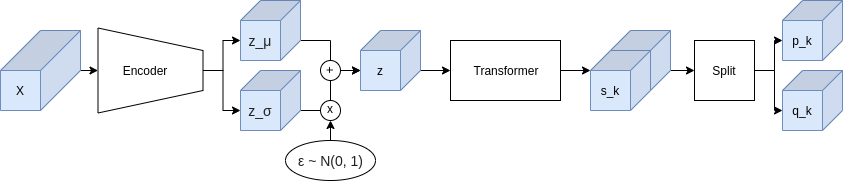
\includegraphics[width=\textwidth]{pictures/HGN_Architecture.png}
\caption{HGN network architecture to find the final abstract position and momentum ($\bm{q}_k$, $\bm{p}_k$) from the input sequence. Tensors are represented in blue and operations in black. The encoder takes as input a sequence of $k+1$ frames concatenated along channels and samples the latent variable $\bm{z} \sim q_{\phi}(\bm{z} \vert \bm{x}_0, ..., \bm{x}_k)$ with the reparametrization trick. The transformer network converts $\bm{z}$ into the state $\bm{s}_k = (\bm{q}_k, \bm{p}_k)$ from which the system evolution will be predicted.}
\label{fig:initial_cond}
\end{figure}

\begin{figure}[h]
\centering
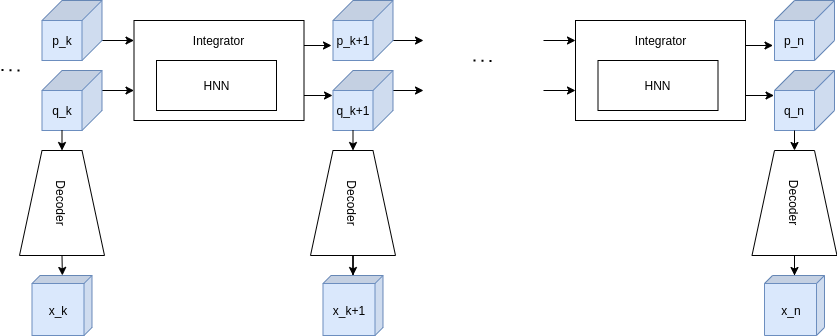
\includegraphics[width=\textwidth]{pictures/rollout_architecture.png}
\caption{Recurrent part of the HGN architecture. Blue cubes represent tensors. The integrator takes the position and momentum for each time-step, computes $\mathcal{H}(\bm{q}_t, \bm{p}_t)$ and computes the abstract state in the next time-step $\bm{s}_{t+1} = (\bm{q}_{t+1}, \bm{p}_{k+1})$ for $t\ge k$ exploiting the Hamiltonian equations of \ref{eq:hamilton}. The decoder takes the abstract position $\bm{q}_{t}$ and decodes it into the original image $\bm{x}_t$.}
\label{fig:unroll}
\end{figure}


\subsection{Integrator Modelling}
\label{sec:integrator_modelling}
%We wondered to what extent it was beneficial for the system to model the Hamiltonian and use its partial derivatives in the integrator. First, computing the partial derivatives is an expensive operation, as it requires to perform backpropagation trough the Hamiltonian Network. Second, our  results and \cite{hgn} show that the resulting Hamiltonian has high variance. We therefore wondered whether the fully-hamiltonian approach is actually helpful, and whether we could achieve the same goal without it.
Since the Hamiltonian network always requires backpropagation, which is an expensive operation, we compare it against a baseline network that does not require backpropagation at evaluation time. We test an architecture almost identical to the HGN, but where the Hamiltonian Network is replaced by a CNN that directly computes $\Delta q$ and $\Delta p$ from $q_t$ and $p_t$. Integration is then performed as an Euler step: $q_{t+1} = q_t + \Delta t \Delta q$ and $p_{t+1} = p_t + \Delta t \Delta p$. In this architecture, therefore, we do not learn Hamiltonian-like dynamics anymore, but we directly learn the system dynamics in the abstract space. This approach achieves a similar reconstruction loss than HGN\cite{hgn}.
%and is still able to operate at different time-scales using a different $\Delta t$.
Results are presented in the additional experiments section.  \ref{sec:additional_experiments}.


\subsection{Datasets} \label{sec:data}
% Describe the datasets you used and how you obtained them.

The datasets considered by the original authors consist of observations of the time evolution of four physical systems: mass-spring, simple pendulum, and two-/three-body systems \cite{hgn}. Since the datasets are not available to us, we re-implement them following as closely as possible the information provided in the paper and by the authors. Moreover, we introduce two new physical systems to experiment with: damped harmonic oscillator and double pendulum (see Figure \ref{fig:datasets}).

The procedure for data generation is analogous to the one used by \cite{hnn}. Given a physical system, we first randomly sample an initial state $(\bm{q}_0, \bm{p}_0)$ in the phase space and generate a $30$ step rollout following the Hamiltonian dynamics. Once the trajectory is obtained, we add Gaussian noise with standard deviation $\sigma = 0.1$ to each phase-space coordinate at each step and render 32x32 image observations. Objects in the systems are represented as circles and we use different colors to represent different objects. We generate 50000 train samples and 10000 test samples for each physical system. To sample the initial conditions $(\bm{q}_0, \bm{p}_0)$, we first sample the total energy denoted as a radius $\bm{r}$ in phase space and then $(\bm{q}_0, \bm{p}_0)$ are sampled uniformly on the circle of radius $\bm{r}$. Note that here $\bm{q}$ and $\bm{p}$ represent the actual positions and momenta vectors of the bodies in the system. These are only used to generate the sequence of images and are not made available to the HGN architecture. The trajectories for each environment are computed using the ground-truth Hamiltonian dynamics and SciPy ODE solver \cite{scipy}.

\begin{figure}
    \centering
    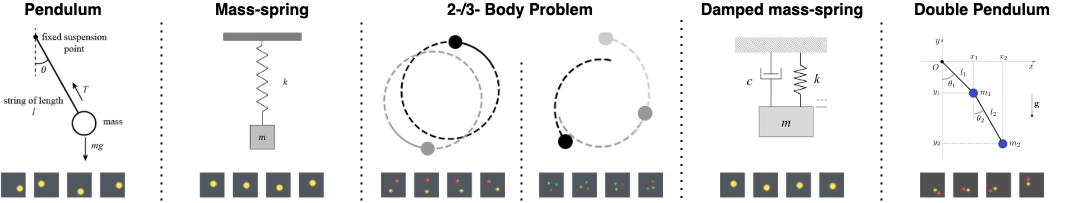
\includegraphics[width=\textwidth]{pictures/data/new_dataset_image.png}
    \caption{Representation and samples from the different physical systems considered in our experiments. Notice that differing from \cite{hgn}, we also consider a damped mass-spring system and a double pendulum.}
    \label{fig:datasets}
\end{figure}
\paragraph{Mass-spring.} Assuming no friction, the Hamiltonian of a mass-spring system is $\mathcal{H} = \frac{p^2}{2m} + \frac{1}{2}kq^2$, where $m$ is the object's mass and $k$ is the spring's elastic constant.
We generate our data considering
$m=0.5$, $k=2$ and $r \sim \mathbb{U}(0.1, 1.0)$.

\paragraph{Pendulum.} An ideal pendulum is modelled by the Hamiltonian $\mathcal{H} = \frac{p^2}{2ml^2} + 2mgl(1 - \cos q)$, where $l$ is the length of the pendulum and $g$ is the gravity acceleration. The data is generated considering $m=0.5$, $l=1$, $g=3$ and $r \sim \mathbb{U}(1.3, 2.3)$.

\paragraph{Two-/three- body problem.} The n-body problem considers the gravitational interaction between $n$ bodies in space. Its Hamiltonian is $\mathcal{H} = \sum_i^n \frac{||\textbf{p}_i||^2}{2m_i} - \sum_{i\neq j}^n \frac{gm_im_j}{||\textbf{q}_i - \textbf{q}_j||}$, where $m_i$ corresponds to the mass of object $i$. In this dataset, we set $\{m_i = 1\}_{i=1}^n$ and $g=1$. For the two-body problem, we modify the observation noise to $\sigma = 0.05$ and set $r\sim\mathbb{U}(0.5, 1.5)$. When considering three bodies, we set $\sigma=0.2$ and $r\sim\mathbb{U}(0.9, 1.2)$.

\paragraph{Dobule pendulum} The double pendulum consists of a system where we attach a simple pendulum to the end of another simple pendulum. For simplicity, we conider both simple pendulums with identical properties (equal mass and length). The Hamiltonian of this system is $\mathcal{H} = \frac{1}{2ml^2}\frac{p_1^2 + p_2^2 + 2p_1p_2cos(q_1 - q_2)}{1 + sin^2(q_1 - q_2)} + mgl\Big(3 - 2\cos q_1 - \cos q_2\Big)$, where $\{q_1, p_1\}$ and $\{q_2, p_2\}$ refer to the phase state of the first and second pendulum respectively. Our data is generated by setting $m=1$, $l=1$, $g=3$ and $r\sim\mathbb{U}(0.5, 1.3)$. In this scenario we consider a very low intense source of noise $\sigma = 0.05$.

\paragraph{Damped oscillator} The damped mass-spring system is obtained by considering a dissipative term in the equations of motion of the ideal mass-spring system. For such systems, one can obtain its dynamics using the Caldirola-Kanai Hamiltonian $\mathcal{H} = e^{\gamma t}\Big(\frac{p^2}{2m} + \frac{1}{2}kq^2 \Big)$ \cite{segovia2018one}, where $\gamma$ is the damping factor of the oscillator. In our experiments, we consider an underdamped harmonic oscillator and set $\gamma=0.3$, $m=0.5$, $k=2$, $r\sim\mathbb{U}(0.75, 1.4)$ and $\sigma=0.1$.


\subsection{Hyperparameters}
We set the same hyperparameters for all experiments as the original paper \cite{hgn} except for GECO parameters, which were not included.
Thus, we perform a grid search on each environment to find the most adequate ones (see Section \ref{sec:hyperparam_search}).

% \subsection{Experimental setup}
% \label{sec:experiments}
% Explain how you ran your experiments, e.g. the CPU/GPU resources and provide the link to your code and notebooks. 

\subsection{Computational requirements}
% Provide information on computational requirements for each of your experiments. For example, the number of CPU/GPU hours and memory requirements. You'll need to think about this ahead of time, and write your code in a way that captures this information so you can later add it to this section. 
A standard training of 50K train samples using the Leapfrog integrator takes around 4 hours on an RTX 2080T GPU and requires around 1910MB.